\chapter{Herramientas}\label{cap.herramientas}
En este capítulo se van a explicar los diferentes interfaces softwares que se van a emplear, así como los lenguajes de programación de los que haremos uso.

Como lenguajes de programación hay que decir que se ha hecho uso de \textit{Python} y \textit{C++}. Para el desarrollo del modelo de Deep Learning que se empleará para la detección, se han realizado pruebas con TensorFlow, Keras y Darknet. OpenCV se ha usado para todo lo relacionado con el tratamiento de imágenes.

La interfaz desarrollada, se ha hecho con gtkmm, herramienta que permite crear interfaces de usuario con múltiples funcionalidades.

Finalmente la evaluación de toda nuestra interfaz en general se ha realizado con DetectionSuite.



\section{DetectionSuite}
En este proyecto se ha hecho uso de la herramienta DetectionSuite~\cite{detectionsuite} para evaluar los resultados de las redes neuronales entrenadas y de nuestra aplicación en general.

DeepLearningSuite es una herramienta que permite evaluar diferentes tipos de redes neuronales sobre un conjunto de datos. La idea es ofrecer una infraestructura genérica para evaluar los algoritmos de detección de objetos contra un conjunto de datos y calcular las estadísticas más comunes:
\begin{itemize}
    \item Intersecion Over Union (IOU)
    \item Precision
    \item Recall
\end{itemize}

La Intersección sobre la Unión (IoU) en la detección de objetos, mide la precisión de un detector en un conjunto de datos en particular y sigue la siguiente fórmula:

\begin{equation}\label{iou}
IoU = \frac{AreaofOverlap}{AreaofUnion}
\end{equation}

Donde AreaofOverlap es el área que pertenece a la intersección entre la predicción y la realidad, mientras que AreaofUnion es el área suma de la predicción y la realidad.

En la Figura\ref{fig.ejemplo_iou} se puede ver un ejemplo visual del ground-truth y la predicción obtenida. En este caso el AreaofOverlap es el área que incluye únicamente la intersección entre lo que hemos predecido y el ground-truth. Y el AreaofUnion es el área que se forma entre el ground-truth y la predicción.

\begin{figure}[H]
  \begin{center}
    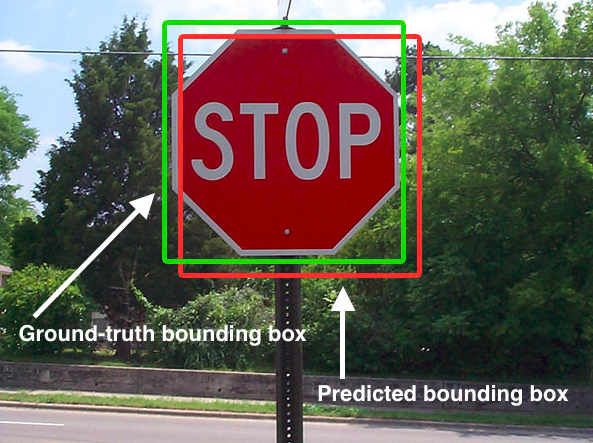
\includegraphics[width=0.6\textwidth]{figures/Herramientas/iou.png}
		\caption{Ejemplo de IoU}
		\label{fig.ejemplo_iou}
		\end{center}
\end{figure}

En la Figura\ref{fig.formula_iou} se ve de forma muy ilustrativa la fórmula comentada anteriormente \ref{iou}.

\begin{figure}[H]
  \begin{center}
    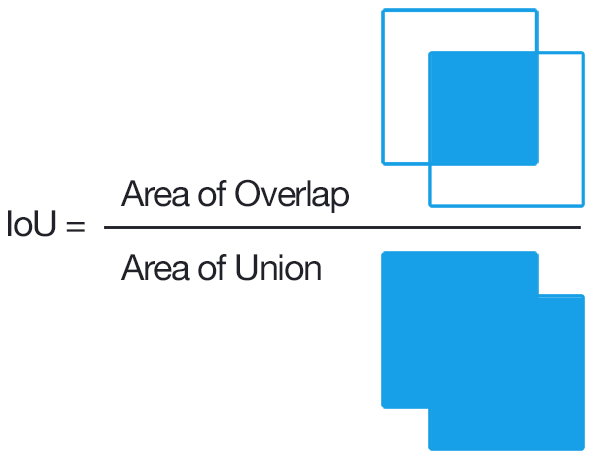
\includegraphics[width=0.4\textwidth]{figures/Herramientas/iou_formula.png}
		\caption{Fórmula IoU}
		\label{fig.formula_iou}
		\end{center}
\end{figure}

Antes de explicar la precisión y el recall hay que aclarar algunos terminos empleados a la hora de evaluar los resultados de las detecciones. A continuación se enumeran algunos necesarios de conocer para entende el recall y la precisión:

\begin{itemize}
    \item True Positive (TP): son los verdaderos positivos, es decir aquellas detecciones que se han hecho correctamente.
    \item False Positive (FP): falsos positivos. Son aquellas detecciones que se han hecho pero son erróneas.
    \item False Negative (FN): falsos negativos. Es la proporción de casos positivos que la prueba detecta como negativos, es decir objetos que no se han detectado y deberían haberse detectado.
    \item True Negative (TN): verdadero negativo. Se refiere a los boundingbox que no deben detectarse en la imagen y no se han detectado. Este valor no se emplea en las métricas.
\end{itemize}

La precisión se trata del total de detecciones correctas entre la cantidad de detecciones obtenidas. La precisión que obtiene DetectionSuite es la promediada (AP),es decir que solo se calcula para aquellas predicciones que tienen un IoU mayor que un umbral (0.5).

\begin{equation}\label{precision}
Precision = \frac{TP}{TP + FP}
\end{equation}

El recall es la cantidad de detecciones correctas entre la cantidad de detecciones reales, es decir las detecciones del ground-truth. Al igual que la precisión, se obtiene un promediado (AR) de las detecciones que tienen un IoU superior a 0.5.

\begin{equation}\label{recall}
Precision = \frac{TP}{TP + FN}
\end{equation}

Volviendo a DetectionSuite, es una herramienta que puede emplearse tanto en Linux como en MacOS. Permite evaluar modelos entrenados en Tensorflow, Keras, Caffe y Darknet. Los formatos de dataset que admite son: \acrshort{yolo}, \acrshort{coco}, ImageNet
Pascal VOC, etc. A continuación se enumeran las entradas soportada:

\begin{itemize}
    \item WebCamera/ USB Camera
    \item Videos
    \item Streams from ROS
    \item Streams from ICE
    \item JdeRobot Recorder Logs
\end{itemize}

En este \acrshort{tfm} en concreto se va a hacer uso de la herramienta AutoEvaluator de DetectionSuite, la cual es capaz de evaluar múltiples redes en un solo conjunto de datos o múltiples conjuntos de datos en una sola ejecuación. Todo lo que necesita es un archivo de configuración que contenga detalles sobre los conjuntos de datos y las redes. Los resultados se escriben en archivos CSV en el directorio de salida especificado.

\section{TensorFlow}
Para el desarrollo de la red neuronal que queremos aplicar en nuestro \textit{smart-traffic-sensor} se  han probado diferentes plataformas de desarrollo de Deep Learning, entre ellas TensorFlow.

TensorFlow\footnote{https://www.tensorflow.org/} es una plataforma de código abierto end-to-end para el machine learning que fue liberada bajo licencia de Apache 2 a finales de 2015 y que está disponible en github~\cite{github_tensorflow}. Fue desarrollada por el equipo de investigación en Machine Learning “Google Brain” en C++ y Python, y es usado en multitud de productos y servicios de Google como Gmail o Google Translation. Google ofrece en su plataforma Cloud ejecutar Tensorflow en Tensor Processing Unit (TPU), un nuevo tipo de procesadores en Cloud optimizados para ejecutar \acrfull{ia}. TensorFlow está orientado a problemas de Deep Learning y nos permite entrenar y construir redes neuronales. El Deep Learning es un área del Machine Learning que trata de asemejarse al funcionamiento del sistema nervioso humano.

TensorFlow puede correr tanto en CPUs como en GPUs (haciendo uso de \acrfull{cuda}). Está disponible en Linux de 64 bits, MacOS, y plataformas móviles que incluyen Android e iOS. Actualmente es la librería más popular en Deep Learning.

Puede ejecutar de forma rápida y eficiente gráficos de flujo. Un gráfico de flujo está formado por operaciones matemáticas representadas sobre nudos, y cuya entrada y salida es un vector multidimensional o tensor de datos, por este motivo recibe el nombre de TensorFlow.

Las ventajas de este software se extienden a muchas disciplinas a parte de la tecnología. Se emplea en medicina en el tema de imágenes médicas para la detección de tumores por ejemplo, también se usa en la detección y combinación de estilos artísticos en la pintura, etc.

En este \acrshort{tfm} se emplea la versión 1.12.0 de tensorflow.

\section{Keras}

Al igual que se ha empleado TensorFlow como plataforma de desarrollo de la red neuronal, se ha hecho uso de Keras.

Keras\footnote{https://keras.io/} es un framework de alto nivel para el aprendizaje, escrito en Python y capaz de correr sobre los frameworks TensorFlow, \acrshort{cntk}, o Theano. Fue desarrollado con el objetivo de facilitar el proceso de experimentación en redes neuronales de forma rápida y eficiente. Puede correr tanto en CPU como en GPU. Permite crear de forma sencilla y rápida los modelos de las redes neuronales (a través de su facilidad de uso, su modularidad y su extensibilidad). Admite redes convolucionales y redes recurrentes, así como combinaciones de las dos.

Inicialmente fue desarrollada en el proyecto de investigación ONEIROS (Open--ended Neuro--Electronic Intelligent Robot Operating System). Su creador es Fran\c{c}ois Chollet, ingeniero de Google.
En 2017, el equipo de TensorFlow de Google decidió dar soporte a Keras en la biblioteca de core de TensorFlow.

Al igual que TensorFlow, Keras se encuentra en github~\cite{keras_github}, pues es de código abierto. Con Keras puedes realizar redes neuronales de forma sencilla y con muy pocas líneas de código, a diferencia de TensorFlow que es algo más complejo. 

Las principales ventajas de Keras son que es fácil de usar, modular, y relativamente fácil de extender, haciendo muy simple su uso.

En este proyecto se hace uso de la versión 2.2.4 de Keras.


\section{Darknet}

Darknet\footnote{https://pjreddie.com/darknet/} es un framework para redes neuronales de código abierto escrito en C y \acrshort{cuda}. Es rápido, fácil de instalar y admite el empleo de CPU y GPU. El código se puede encontrar en github~\cite{darknet_github}.

Darknet se creo con el fin de emplearse en el diseño, ejecución y entrenamiento de redes neuronales profundas para la clasificación y detección de objetos. 

Las principales ventajas de este sistema son su simplicidad en términos de uso y su tama\~{n}o reducido.

En nuestro proyecto haremos uso de \acrfull{yolo}, que es un sistema de detección de objetos que funciona sobre Darknet. \acrshort{yolo} utiliza deep learning y \acrshort{cnn} para detectar objetos, y se distingue de sus competidores porque requiere de ver la imagen una sola vez, permitiéndole ser mucho más rápido que el resto del algoritmos. Gracias a su gran rapidez es capaz de detectar objetos en tiempo real en videos (hasta 30 FPS).

A la hora de realizar la detección, \acrshort{yolo} en primer lugar divide la imagen en una cuadrícula de SxS. En cada una de sus celdas se estiman sus N posibles bounding boxes  con sus respectivas probabilidades de acierto. Teniendo así SxSxN bounding boxes. Aquellas predicciones que tengan una probabilidad por debajo de un umbral quedarán eliminadas. A las que superen dicho umbral se les aplicará \textit{non--max suppression}, lo cual sirve para eliminar objetos detectados por duplicado. Este proceso puede verse en la siguiente Figura\ref{fig.yolo}.

\begin{figure}[H]
  \begin{center}
    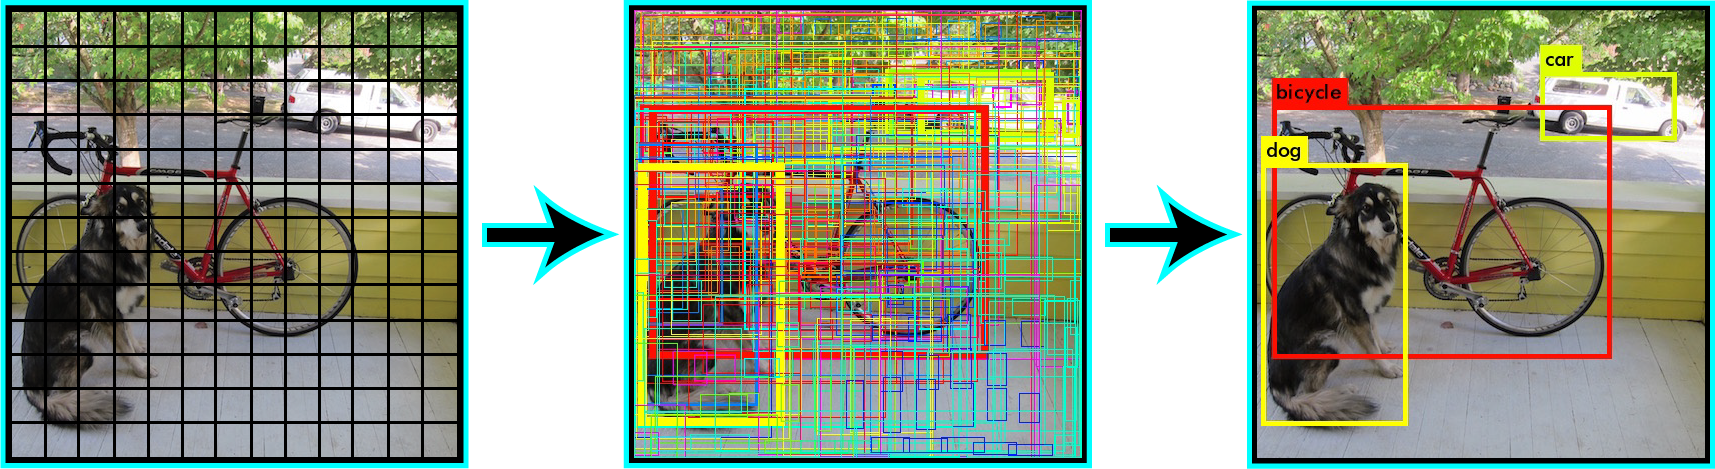
\includegraphics[width=0.9\textwidth]{figures/Herramientas/yolo.png}
		\caption{Proceso de Yolo}
		\label{fig.yolo}
		\end{center}
\end{figure}

En este \acrshort{tfm} se ha usado Darknet para el desarrollo de una red neuronal. La versión que se ha empleado es \textit{YOLOv3}, es decir, la última versión existente.

\section{Biblioteca OpenCV}

\textit{OpenCV}\footnote{https://opencv.org/} es una librería de código abierto desarrollada por Intel y publicada  bajo licenciade BSD. Esta librería implementa gran variedad de herramientas para la interpretación de la imagen. Sus  siglas  provienen  de  los  términos anglosajones ``Open Source Computer  Vision Library", y tal y como se puede deducir es una librería destinada a aplicaciones de visión por computador en tiempo real. Puede ser empleada en MacOS, Windows y Linux,y existen versiones para \textit{C\#}, \textit{Python} y \textit{Java}, a pesar de que originalmente era una librería en \textit{C/C++}. Además hay interfaces para \textit{Ruby}, \textit{Python}, \textit{Matlab} y otros lenguajes. 

\textit{OpenCV} es una librería que implementa algoritmos para técnicas de calibración, detección de rasgos, rastreo, análisis de la forma, análisis del movimiento, reconstrucción 3D, segmentación de objetos y reconocimiento, etc. Los algoritmos se basan  en  estructuras de datos flexibles acopladas con estructuras IPL  (Intel  Image Processing Library),aprovechándose de la arquitectura de Intel en la optimización de más de las mitad de las funciones.

Incorpora funciones básicas para modelar el fondo, sustraer dicho  fondo y generar imágenes de movimiento MHI  (Motion  History  Images).  Además  incluye  funciones para determinar dónde hubo movimiento y en qué dirección. 

\begin{figure}[H]
  \begin{center}
    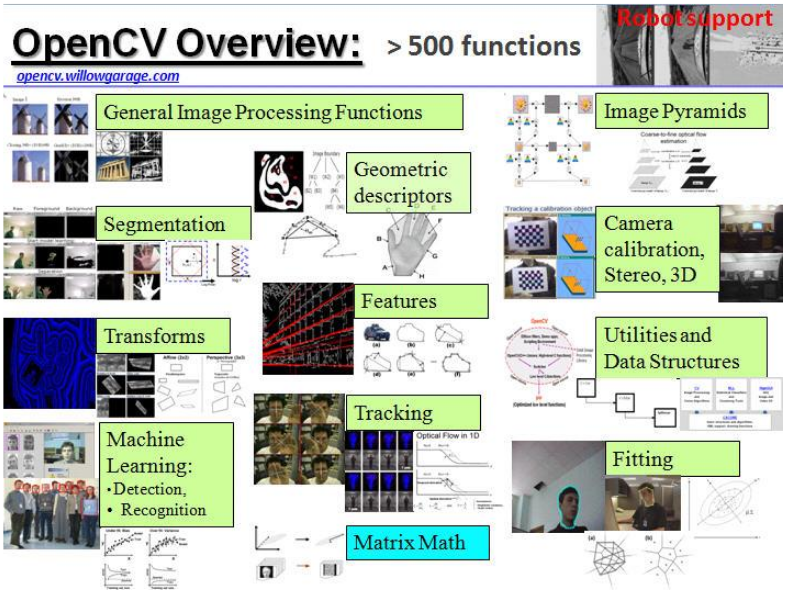
\includegraphics[width=0.6\textwidth]{figures/Herramientas/opencv.png}
		\caption{Funciones de OpenCV}
		\label{fig.opencv}
		\end{center}
\end{figure}

Fue diseñado para tener una alta eficiencia computacional, está escrito en C y puede aprovechar las ventajas de los procesadores multinúcleo. Contiene más  de  2500  funciones  que  abarcan  muchas  áreas  de  la  visión  artificial.  También  tiene  una librería   de   aprendizaje   automático   (MLL,   Machine   Learning   Library)   destinada   al reconocimiento  y agrupación de patrones estadísticos.

Desde su aparición OpenCV ha sido usado en numerosas aplicaciones. Entre las cuales se encuentran la unión de imágenes de satélites y mapas web, la reducción de ruido en imágenes  médicas,  los  sistemas  de  detección  de movimiento,  la  calibración  de  cámaras,  el manejo  de  vehículos  no  tripulados, el  reconocimiento  de  gestos, etc. OpenCV  es  empleado también  en  reconocimiento  de  música  y  sonido,  mediante  la  aplicación  de  técnicas  de reconocimiento de visión en imágenes de espectrogramas del sonido.

Hay  una  gran  cantidad  de  empresas    y  centros  de  investigación  que  emplean  estas técnicas como IBM, Microsoft, Intel, SONY, Siemens, Google, Stanford, MIT, CMU, Cambridge e INRIA.

En este proyecto se hace uso de la versión \textit{OpenCV} 3.2.

\section{Lenguaje C++}

El lenguaje \textit{C++} nació en el laboratorio ATT, pero no surgió oficialmente hasta 1983, ya  que  fue  entonces  cuando  comenzó  a  usarse.  Fue  creado  por  Bjarne  Stroustrup,  el  cual comenzó con \textit{C++} en 1980. 

Este lenguaje en un principio se llamaba \textit{C} con clases, pues se diseñó conservando la mayoría de los conceptos de C y se añadieron características como por ejemplo clases. \textit{C++} se  desarrolló  a  partir  de  \textit{C}  y por tanto lo incluye. Esta  parte  de  \textit{C}  incluida se  llama  \textit{C-} y  puede compilarse como \textit{C++}.

Debido  al  gran  éxito  que  obtuvo  entre  los programadores,  la  ATT  comenzó  a estandarizarlo   internamente   en   1987. Y   en   1989   se   formó   un   comité   ANSI   para estandarizarlo a nivel americano e internacional.

\textit{C++}   es   un   lenguaje   híbrido   que   ha   tomado   todas   las   características   de   la programación  orientada  a objetos y  mejora  las  capacidades  de  \textit{C}. Es muy versátil y potente, por ello ocupa el primer puesto como herramienta de desarrollo de aplicaciones.

\section{Lenguage Python}

\textit{Python}\footnote{https://www.python.org/} es un lenguaje de programación de alto nivel, muy fácil de aprender y de código abierto. \textit{Python Software Foundation} es quien administra este lenguaje actualmente.

La primera versión surgió en 1901, pero no fue publicada hasta tres años después. Su creador fue Guido van Rossum, un investigador holandés, el cual trabaja en el centro de investigación CWI (Centrum Wiskunde \& Informatica).

Este lenguaje incluye numerosas funcionalidades como el manejo de excepciones, la orientación a objetos, diccionarios, listas, etc. Dispone de módulos que permiten el uso de sockets, entrada y salida de ficheros, e incluso interfaces gráficas como Qt. Todo ello se creó con el objetivo de que fuera fácil de entender y emplear, pero sin perder funcionalidades que pueden ofrecer lenguajes más complejos como C. Al ser un lenguaje interpretado, no es necesario compilar el código.

Por compatibilidad con la versión original de \textit{smart-traffic-sensor} se ha empleado la versión 2.7.12 de \textit{Python}.

\section{Gtkmm}

\textit{Gtkmm}\footnote{http://www.gtkmm.org} es una encapsulación en \textit{C++} de \textit{Gtk+}. Dicha encapsulación ofrece todos los beneficios de la orientación a objetos, e incorpora otras cualidades como una mejora en la comprobación de tipos, código más reducido y legible, y un menor uso de los punteros. 

Se trata de un \textit{toolkit} para desarrollar interfaces gráficas de usuario. Es un software libre distribuido bajo la Licencia Pública General Reducida de GNU (LGPL).

\textit{Gtkmm} se organiza por medio de ventanas, las cuales contienen \textit{widgets}, como por ejemplo botones etiquetas,cuadros de texto, etc.  Para cada widget debemos tener un objeto C++ con el cual controlar su funcionamiento, es decir si por ejemplo nuestro widget es un botón, necesitaremos funciones para saber si se ha pulsado o no, y acerca de que realizar si se hubiera pulsado, para todo ello se emplea un objeto de C++. 

Aunque se puede especificar el diseño y apariencia de las ventanas y widgets con C++, resulta más conveniente usar \textit{Glade} para el diseño de la interfaz de usuario y cargarlos en tiempo de ejecución con \textit{Gtk::Builder}. Con  \textit{Glade} podemos desarrollar las interfaces de usuario, guardarlas en formato .glade y luego cargarlas desde \textit{gtkmm} empleando \textit{ Gtk::Builder}.

En este caso se hace uso de la versión \textit{gtkmm}3.0.



